\section{Related work}
 
Several projects have been tested to represent the idea of image recognition. For example,  according to an abstract article from the book Automation in Construction, computer vision has experimented with construction projects in Wuhan, China \cite{Luo}. They use Convolutional Neural Network (CNN) to record and detect the activities of construction workers. The goal of this observation is for the supervisors to verify that the projects and jobs are done accordingly.

Also, two articles discuss how CNN works, and what computer vision exactly is. They discuss challenges that require taking light, deformity of objects, hidden images, 2 or 3-dimensional figures, and a variety of dynamics into consideration \cite{Bansac}. Although these challenges experiment with computer vision. The articles thoroughly explain how convolutions take place in identifying numerous dimensional layers and set a pool of filters to collect information.

\begin{figure}
    \centering
    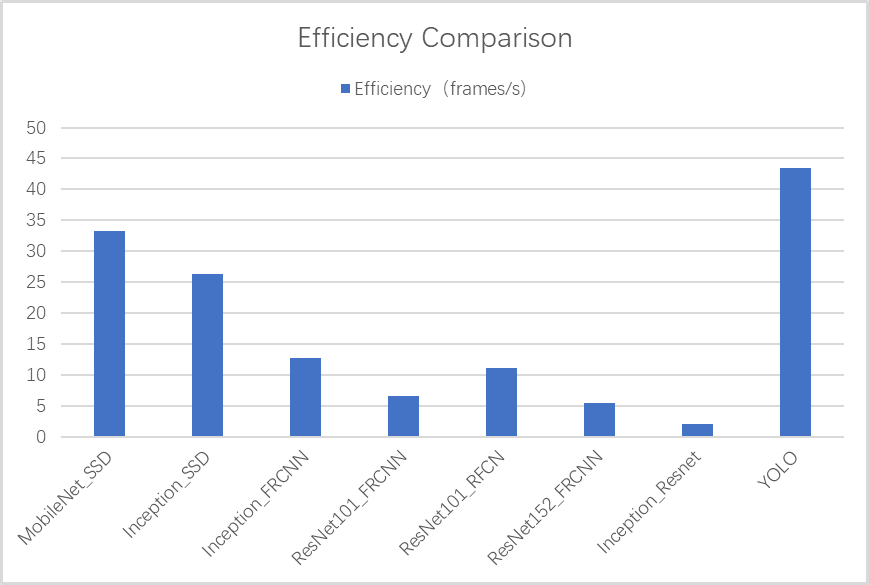
\includegraphics[width=6cm]{Security Object Detection, Surveillance/Latex/figures/fig3.png}
    \caption{Efficiency Comparison of Eight Groups of Experiments \cite{Xie}}
    \label{fig:fig1}
\end{figure}

A Tutorial used to assist in the creation of the experiment with the raspberry pi object detection was a blog by Leigh Johnson written by Adrian Rosebrock, “Real-time Object Tracking with TensorFlow, Raspberry Pi, and Pan-Tilt HAT”, in which she describes the materials used to create the object detector. She discussed the assembly of a TensorFlow Lite model called MobileNetV3-SSD attached to a Raspberry Pi. She also explained how the tracking was implemented onto the design, by using a proportional-integral-derivative controller(PID) controller. To accomplish the detector she also implemented an accelerator using Coral's USB Edge TPU Accelerator and the Edge TPU Compiler \cite{Johnson}. Before continuing the tutorial she provides a detailed list of terms that assists the reader in understanding each term by providing definitions, such as MobileNetV3, a computer vision model in which is resourceful for mobile phone processors. As seen in figure \ref{fig:fig1}, Mobilnet is very efficient compared to when compared to others. The setup provided benchmark data of an estimated 7 to 8 frames per second. She added a custom operation TFLite\_Detection\_PostProcess that implements a technique called Non-Maximum Suppression, which filters multiple box proposals \cite{Johnson}. This although not planned to experiment with presently, is still something the team plans to experiment and implement for further advanced research and testing.

A better tutorial closer to the experiment we did is “How to perform Object Detection with TensorFlow Lite on Raspberry Pi” by Shawn Hymel, which describes a setup using coco as the MobileNetV1, just as described in the previous tutorial. Since this tutorial actually uses COCO as the team planned to experiment with, this one makes it a closer method almost identical to the one implemented. COCO is described as a collection of a variety of figures labeled by multiple companies like Microsoft and universities specialized in research of computer vision \cite{Hymel}. Just like the previous design this one also uses TensorFlow Lite, Linux, Python, and a Raspberry Pi. However, instead of using MobileNetV3, MobileNetV1 is used. They also describe different versions of the Raspberry Pi used, this is helpful because they explain how each works, but one stands out the most for having a faster processor and more memory implemented on the small computer board. Raspberry Pi 4B is recommended for its processing speed and memory, compared to Raspberry Pi 3B \cite{Hymel}. Raspberry Pi 3B tends to give you a smaller amount of frames per second, compared to the 5 frames per second for the Raspberry Pi 4B, either 4 gigabytes or 8 gigabytes work.
